\documentclass{article}
\usepackage{amsmath}
\usepackage{amssymb}
\usepackage{amsbsy}
\usepackage{bbm}
\usepackage{url}
\usepackage{color}
\usepackage{float}
\usepackage{graphicx}
\usepackage{epstopdf}
\usepackage{fancyhdr}
\usepackage{enumerate}
\usepackage{tikz}
\usepackage[ruled,vlined]{algorithm2e}
\usepackage[colorlinks=true,urlcolor=blue]{hyperref}
\usepackage[utf8]{inputenc}
\numberwithin{figure}{section}

% option + cmd + V to view pdf in VScode

\title{CS224W Homework 1}
\author{Stanford}

\newcommand{\Solution}[1]{{\medskip \color{red} \bf $\bigstar$~\sf \textbf{Solution}~$\bigstar$ \sf #1 } \bigskip}
\begin{document}

\maketitle


\section{GNN Expressiveness (28 points)}


\textbf{ For Q1.1, write down number of layers needed. For Q1.2, write down the transition matrix $M$ and the limiting distribution $r$. For Q1.3 and 1.4, write down the transition matrix w.r.t $A$ and $D$. For Q1.5, write down your proof in a few sentences (equations if necessary). For Q1.6, describe the message function, aggregate function, and update rule in a few sentences or equations.}

Graph Neural Networks (GNNs) are a class of neural network architectures used for deep learning on graph-structured data. Broadly, GNNs aim to generate high-quality embeddings of nodes by iteratively aggregating feature information from local graph neighborhoods using neural networks; embeddings can then be used for recommendations, classification, link prediction, or other downstream tasks. Two important types of GNNs are GCNs (graph convolutional networks) and GraphSAGE (graph sampling and aggregation).

Let $G = (V,E)$ denote a graph with node feature vectors $X_u$ for $u \in V$. To generate the embedding for a node $u$, we use the neighborhood of the node as the computation graph. At every layer $l$, for each pair of nodes $u \in V$ and its neighbor $v \in V$, we compute a message function via neural networks, and apply a convolutional operation that aggregates the messages from the node’s local graph neighborhood (Figure \ref{fig:Q4-gnn-architecture}), and updates the node’s representation at the next layer. By repeating this process through $K$ GNN layers, we capture feature and structural information from a node’s local $K$-hop neighborhood. For each of the message computation, aggregation, and update functions, the learnable parameters are shared across all nodes in the same layer.

\begin{figure}[!htb]
\centering
  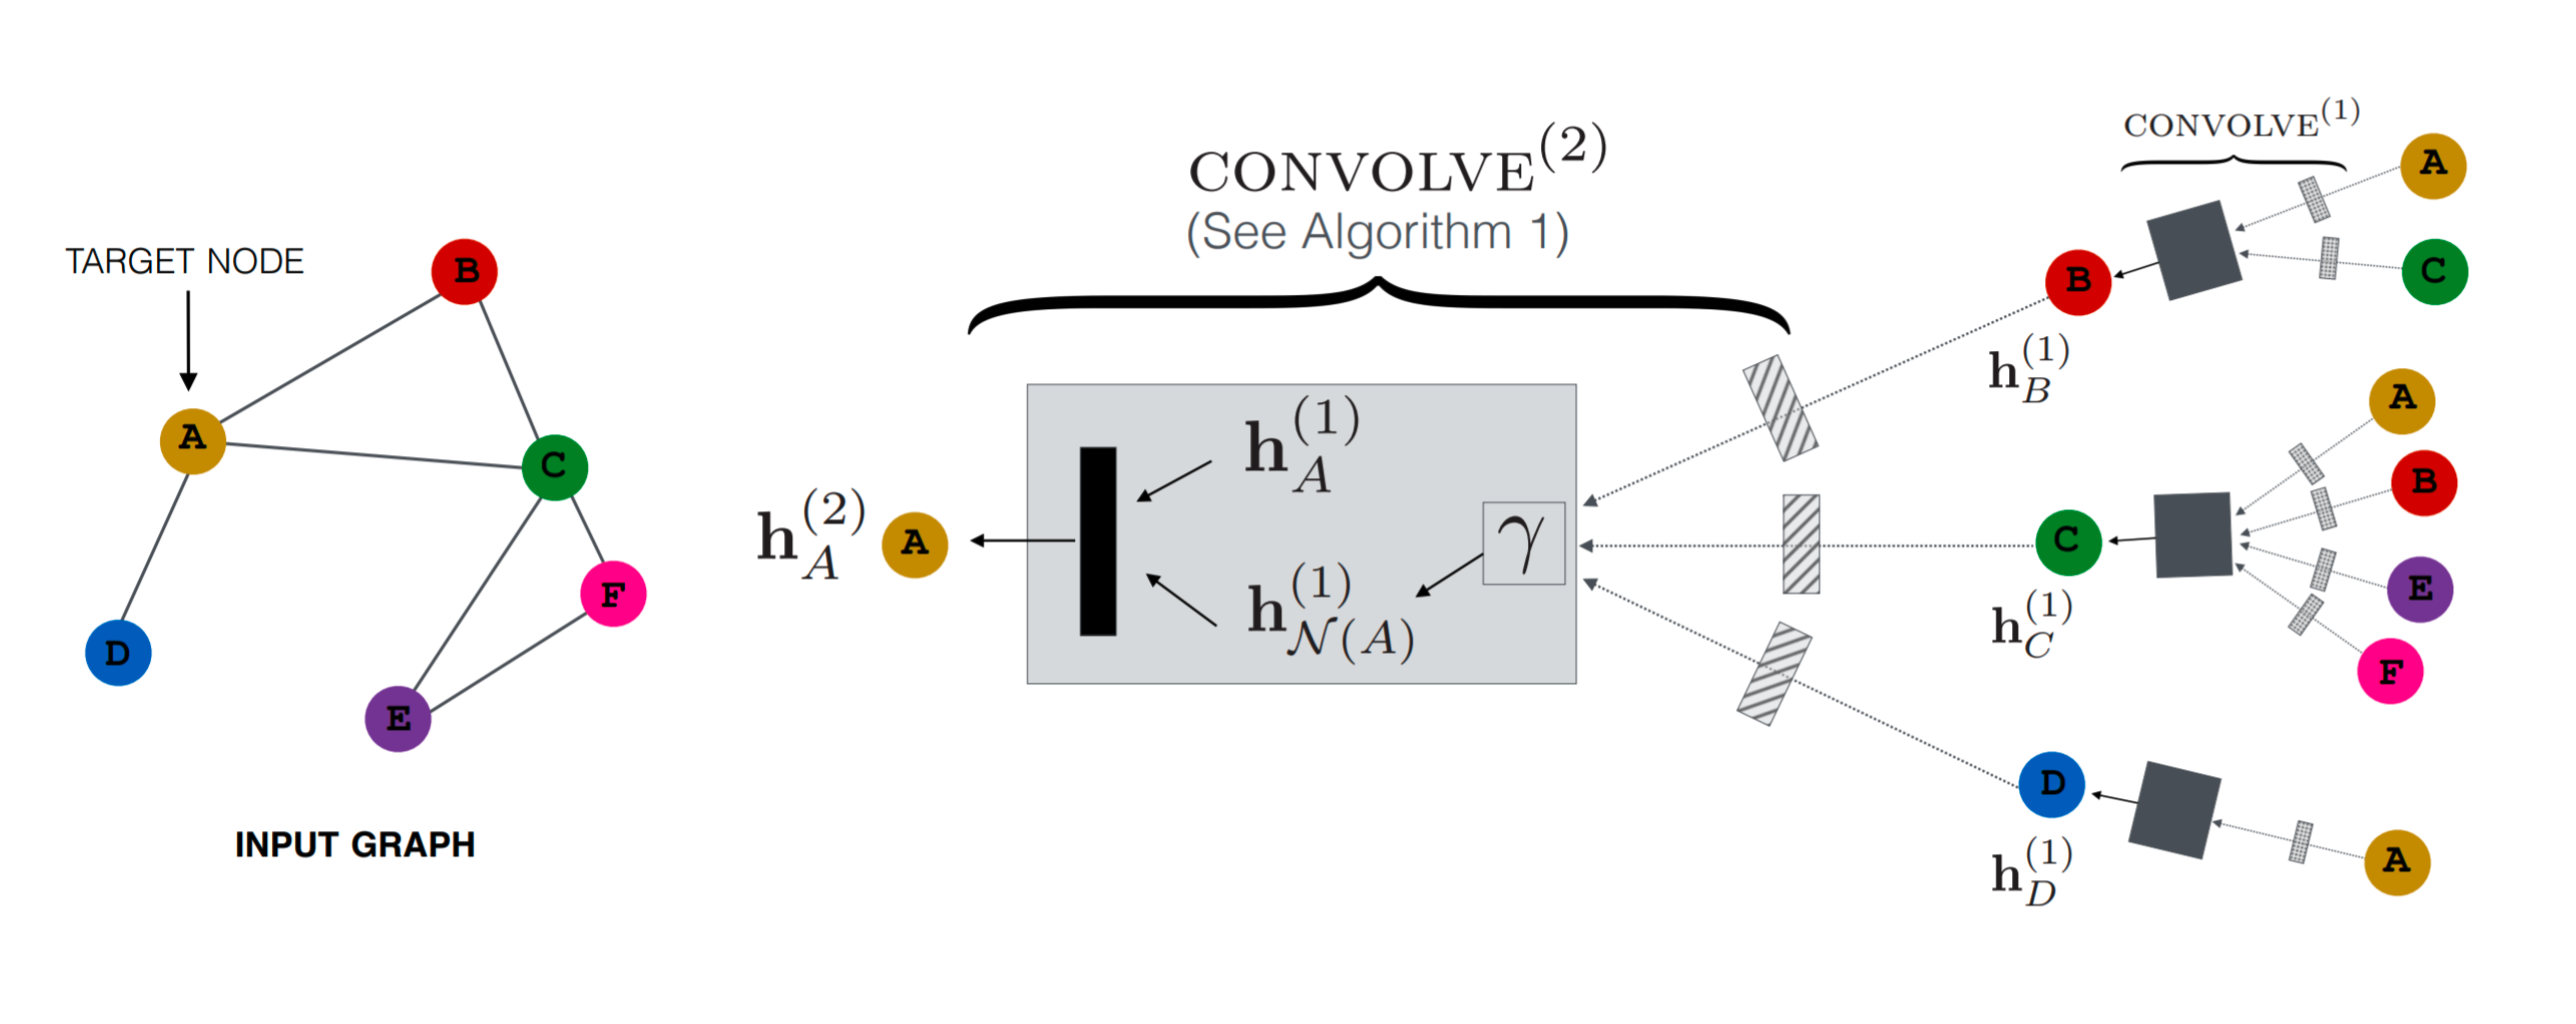
\includegraphics[width=0.7\columnwidth]{CS224W_Homework1/gnn-architecture.png}
  \caption{GNN architecture}   
  \label{fig:Q4-gnn-architecture}
\end{figure}

We initialize the feature vector for node $X_u$ based on its individual node attributes. If we already have outside information about the nodes, we can embed that as a feature vector. Otherwise, we can use a constant feature (vector of 1) or the degree of the node as the feature vector.

These are the key steps in each layer of a GNN:
\begin{itemize}
    \item \textbf{Message computation}: We use a neural network to learn a message function between nodes. For each pair of nodes $u$ and its neighbor $v$, the neural network message function can be expressed as $M(h^k_u,h^k_v,e_{u,v})$. In GCN and GraphSAGE, this can simply be $\sigma(W h_v + b)$, where $W$ and $b$ are the weights and bias of a neural network linear layer. Here $h^k_u$ refers to the hidden representation of node $u$ at layer $k$, and $e_{u,v}$ denotes available information about the edge $(u, v)$, like the edge weight or other features. For GCN and GraphSAGE, the neighbors of $u$ are simply defined as nodes that are connected to $u$. However, many other variants of GNNs have different definitions of neighborhood.
    \item \textbf{Aggregation}: At each layer, we apply a function to aggregate information from all of the neighbors of each node. The aggregation function is usually permutation invariant, to reflect the fact that nodes’ neighbors have no canonical ordering. In a GCN, the aggregation is done by a weighted sum, where the weight for aggregating from $v$ to $u$ corresponds to the $(u,v)$ entry of the normalized adjacency matrix $D^{-1/2}AD^{-1/2}$.
    \item \textbf{Update}: We update the representation of a node based on the aggregated representation of the neighborhood. For example, in GCNs, a multi-layer perceptron (MLP) is used; Graph-SAGE combines a skip layer with the MLP.
    \item \textbf{Pooling}: The representation of an entire graph can be obtained by adding a pooling layer at the end. The simplest pooling methods are just taking the mean, max, or sum of all of the individual node representations. This is usually done for the purposes of graph classification.
\end{itemize}

We can formulate the Message computation, Aggregation, and Update steps for a GCN as a layer-wise propagation rule given by:
\begin{equation}
    h^{k+1} = \sigma(D^{-1/2} A D^{-1/2} h^k W^k)
\end{equation}

where $h^k$ represents the matrix of activations in the $k$-th layer, $D^{-1/2}AD^{-1/2}$ is the normalized adjacency of graph $G$, $W_k$ is a layer-specific learnable matrix, and $\sigma$ is a non-linearity function. Dropout and other forms of regularization can also be used.

We provide the pseudo-code for GraphSAGE embedding generation below. This will also be relevant to the questions below.

\begin{figure}[H]
\centering
  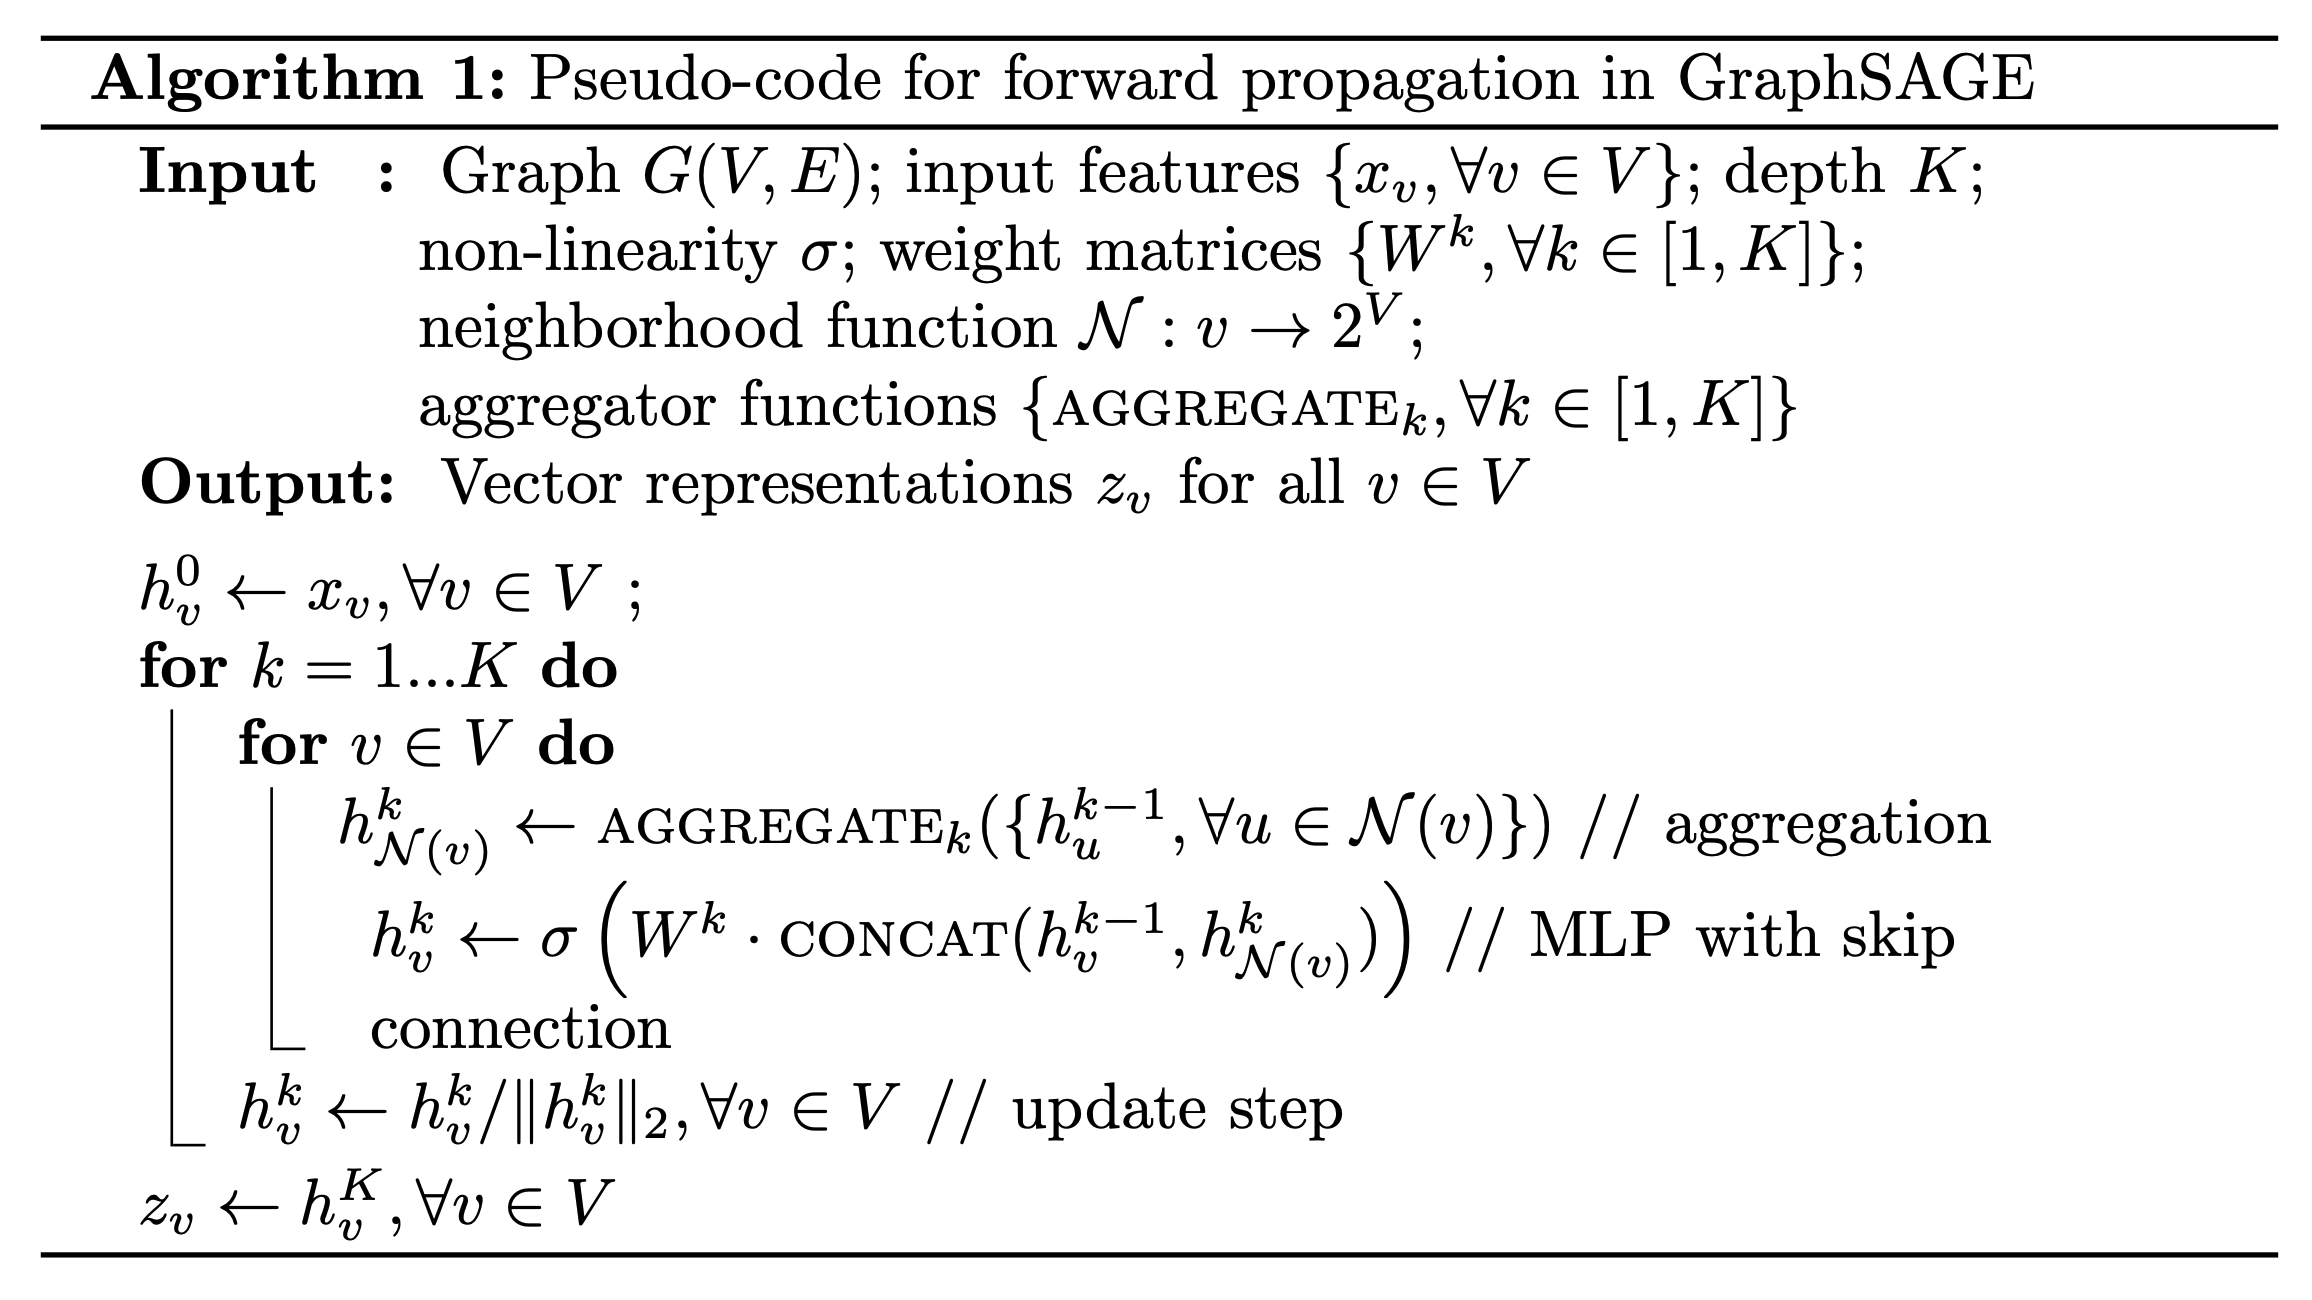
\includegraphics[width=1\columnwidth]{CS224W_Homework1/algorithm.png}
\end{figure}

In this question, we investigate the effect of the number of message passing layers on the expressive power of Graph Convolutional Networks. In neural networks, expressiveness refers to the set of functions (usually the loss function for classification or regression tasks) a neural network is able to compute, which depends on the structural properties of a neural network architecture.

\subsection{Effect of Depth on Expressiveness (4 points)}

\begin{figure}[!htb]
  \centering
    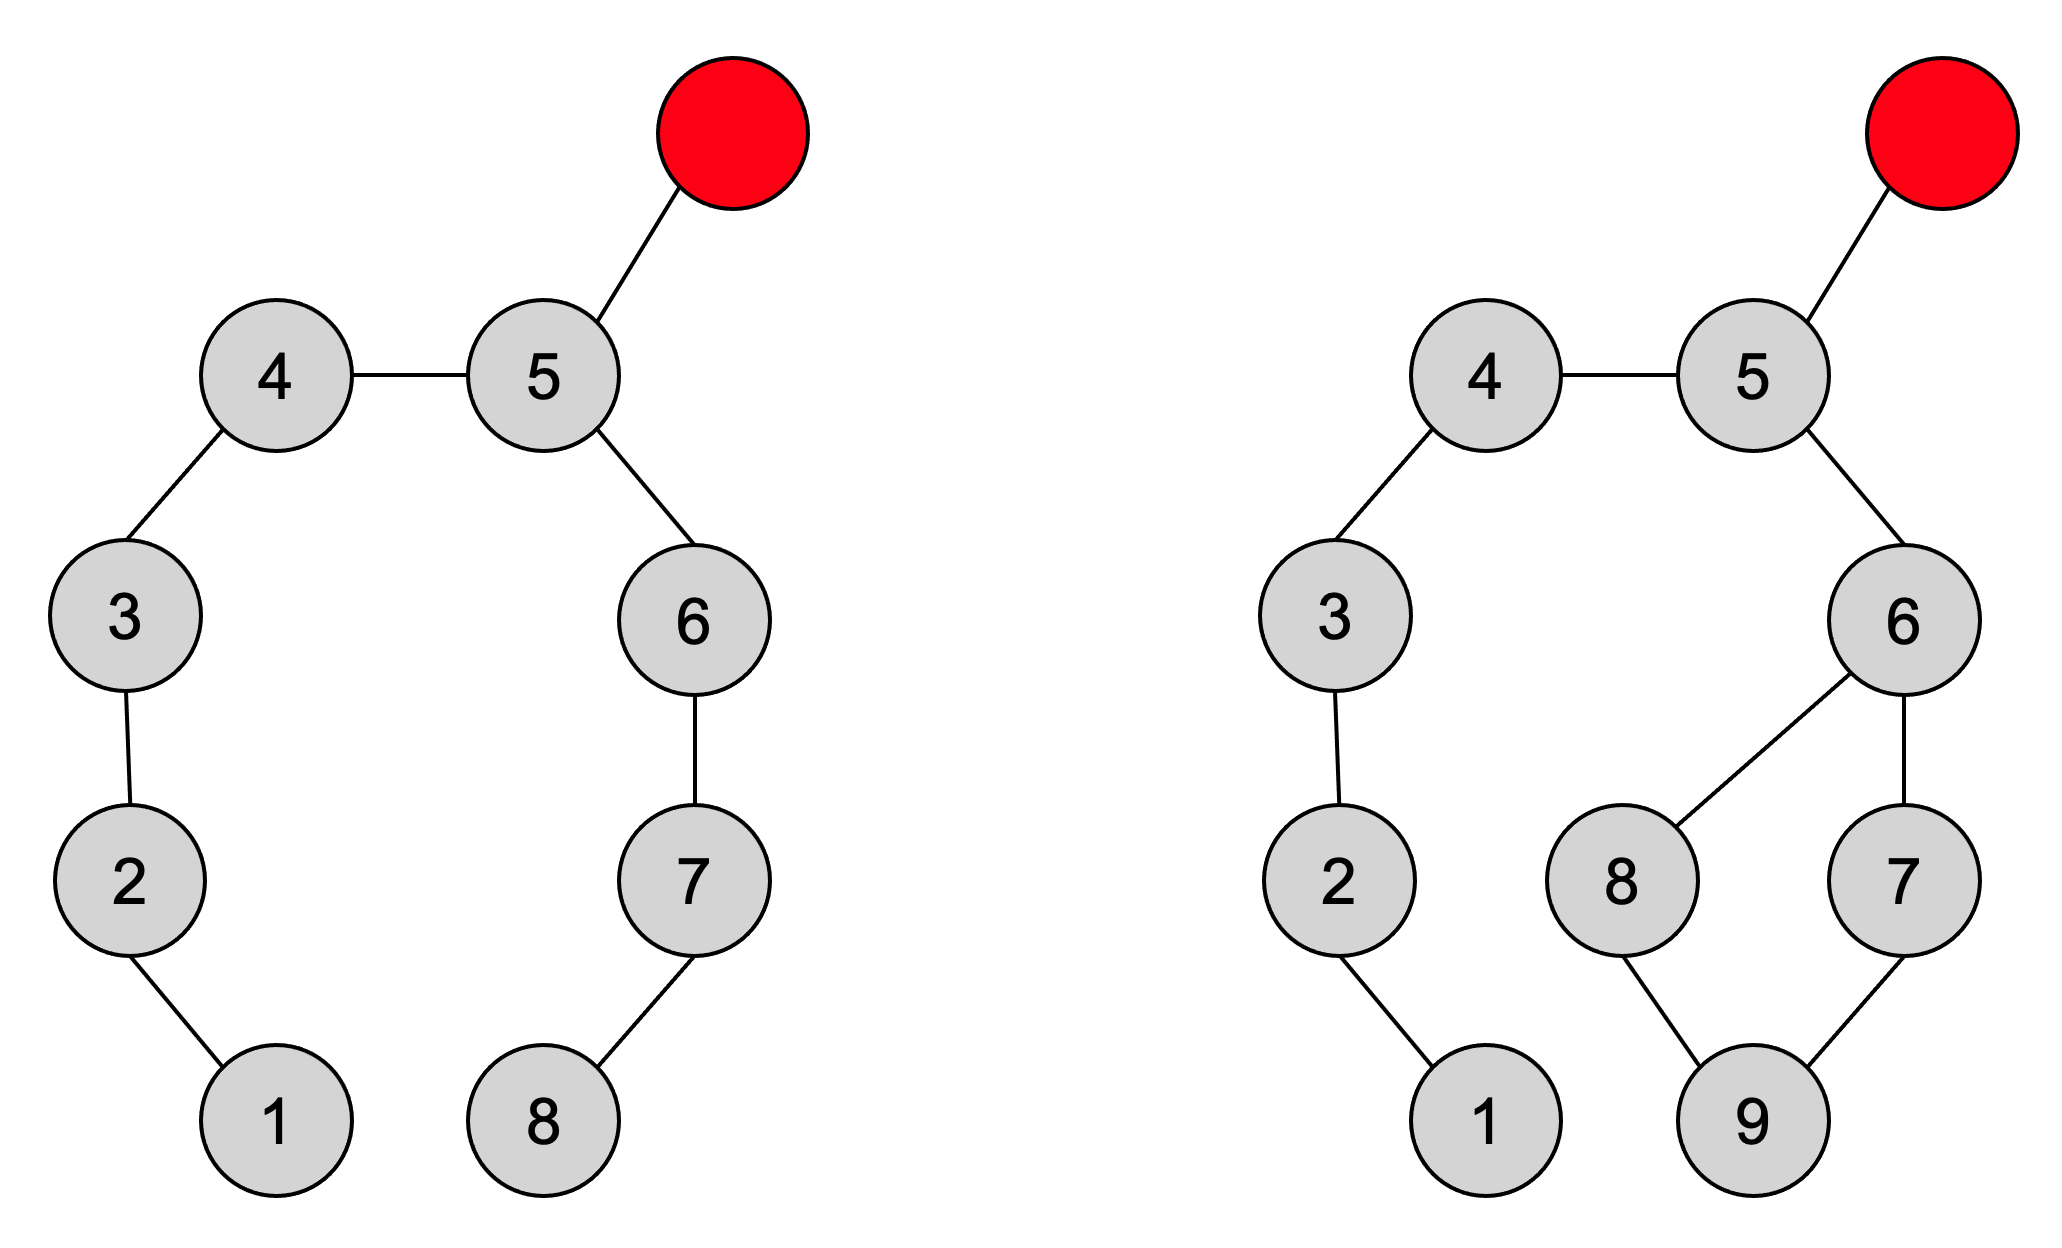
\includegraphics[width=0.6\columnwidth]{CS224W_Homework1/fig4-1.png}
    \caption{Figure for Question 1.1}
    \label{fig:Q4.1}
  \end{figure}
Consider the following 2 graphs in figure~\ref{fig:Q4.1}, where all nodes have 1-dimensional initial feature vector $x = [1]$. We use a simplified version of GNN, with no nonlinearity,
no learned linear transformation, and sum aggregation. Specifically, at every
layer, the embedding of node $v$ is updated as the sum over the embeddings of
its neighbors ($N_v$) and its current embedding $h^t_v$ to get $h^{t+1}_v$. We run the GNN
to compute node embeddings for the 2 red nodes respectively. Note that the 2 red nodes have different 5-hop neighborhood structure (note this is not the minimum number of hops for which the neighborhood structure of the 2 nodes differs). How many layers of message passing are needed so that these 2 nodes can be distinguished (i.e., have different GNN embeddings)? Explain your answer in a few sentences.


.\\

\Solution{3 layers are needed since the 1-hop and 2-hop neighborhoods are the same. The 3-hop neighborhoods for the left and right graphs are \{3, 7\} and \{3, 7, 8\} respectively.
}

\subsection{Random Walk Matrix (4 points)}

Consider the graph shown below (figure~\ref{fig:Q4.2}).
\begin{enumerate}
    \item Assume that the current distribution over nodes is $r = [0,0,1,0]$, and after the random walk, the distribution is $M \cdot r$. What is the random walk transition matrix $M$, where each row of $M$ corresponds with the node ID in the graph?
    \item What is the limiting distribution $r$, namely the eigenvector of $M$ that has an eigenvalue of 1 ($r = Mr$)? Write your answer in fraction form or round it to the nearest thousandth place and in the following form, e.g. $[1.200, 0.111, 0.462, 0.000]$. Note that before reporting you should normalize $r$ (Hint: $r$ is a probability distribution).
\end{enumerate}

\begin{figure}[!htb]
\centering
  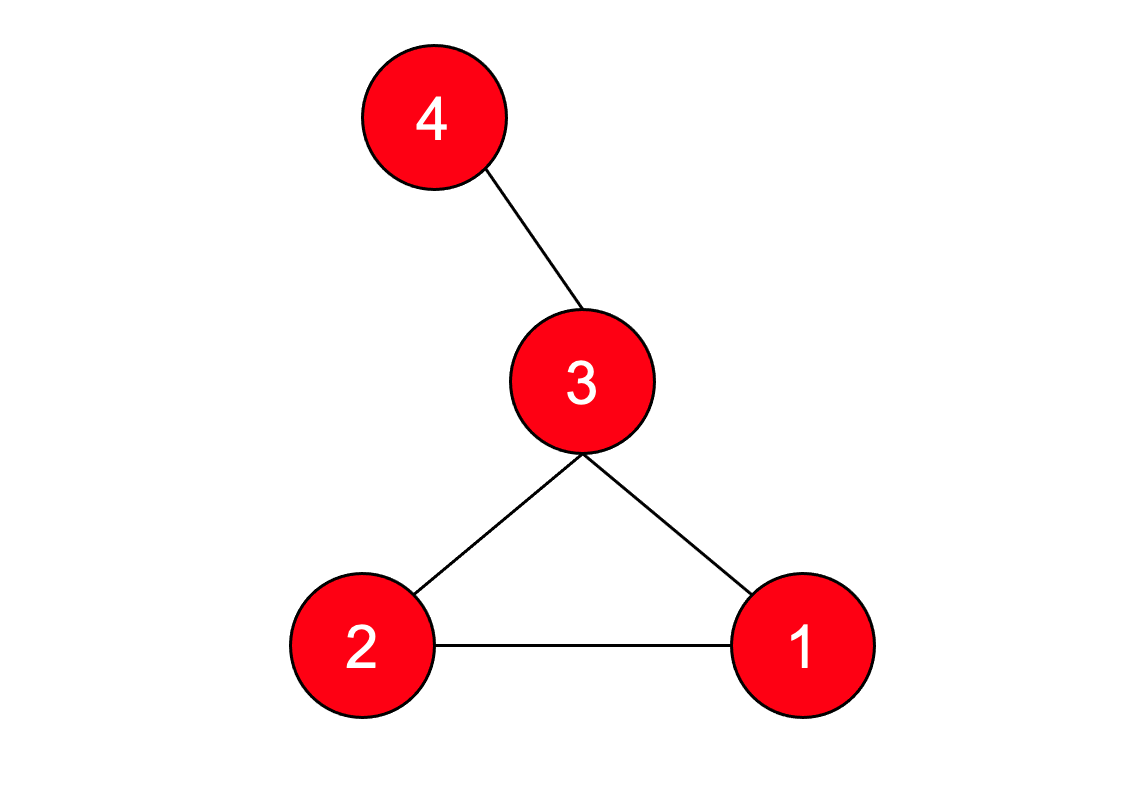
\includegraphics[width=0.5\columnwidth]{CS224W_Homework1/fig4-2.png}
  \caption{Figure for Question 1.2}
  \label{fig:Q4.2}
\end{figure}

\Solution{$r$ tells us the random walk is currently at node 3. $M =$ 
\[
\begin{bmatrix}
  0 & .5 & .5 & 0 \\
  .5 & 0 & .5 & 0 \\
  .33 & .33 & 0 & .33 \\
  0 & 0 & 1 & 0
\end{bmatrix}
\]
The eigenvector corresponding to 1 is $[1,1,1,1]$ and normalized we divide by the number of nodes to get $[.25,.25,.25,.25]$.}



\subsection{Relation to Random Walk (i) (4 points)}

Let’s explore the similarity between message passing and random walks. Let $h^{(l)}_i$ be the embedding of node $i$ at layer $l$. Suppose that we are using a mean aggregator for message passing, and omit the learned linear transformation and non-linearity: $h^{(l+1)}_i = \frac{1}{|N_i|} \sum_{j \in N_i} h^{(l)}_j$. If we start at a node $u$ and take a uniform random walk for 1 step, the expectation over the layer-$l$ embeddings
of nodes we can end up with is $h^{(l+1)}_u$, exactly the embedding of $u$ in the next GNN layer. What is the transition matrix of the random walk? Describe the transition matrix using the adjacency matrix $A$, and degree matrix $D$, a diagonal matrix where $D_{i,i}$ is the degree of node $i$.

\Solution{Let the transition matrix be T. Using the graph in Fig 1.3, we have $T_{uv}=\frac{A_{vu}}{D_{u,u}}$. 
Overall, since from lectures we learnt multiplying by $D^{-1}$ is the same as normalizing, 

we have $T=D^{-1}A$ so that $h^{(l+1)}_i = T \cdot h^{(l)}_j$.}


\subsection{Relation to Random Walk (ii) (4 points)}

Suppose that we add a skip connection to the aggregation from Question 1.3:
$$h^{(l+1)}_i = \frac{1}{2}h^{(l)}_i + \frac{1}{2}\frac{1}{|N_i|} \sum_{j \in N_i} h^{(l)}_j$$
What is the new corresponding transition matrix?

\Solution{We would keep T from before but halve it, and add half the identity matrix since we want to add half of the $h^{(l)}_j$ vector. So $T = \frac{1}{2}I + \frac{1}{2}D^{-1}A$.}


\subsection{Over-Smoothing Effect (5 points)}

In Question 1.1 we see that increasing depth could give more expressive power.
On the other hand, however, a very large depth also gives rise to the undesirable
effect of over smoothing. Assume we are still using the aggregation function
from Question 1.3: $h^{(l+1)}_i = \frac{1}{|N_i|} \sum_{j \in N_i} h^{(l)}_j$. Show that the node embedding $h^{(l)}$ will converge as $l \rightarrow \infty$. Here we assume that the graph is connected and has no bipartite components. We also assume that the graph is undirected.

Over-smoothing thus refers to the problem of node embedding convergence. Namely, if all node embeddings converge to the same value then we can no longer distinguish them and our node embeddings become useless for downstream tasks. However, in practice, learnable weights, non-linearity, and other architecture choices can alleviate the over-smoothing effect.

\textbf{Hint: Think about the Markov Convergence Theorem: Is the Markov chain irreducible and aperiodic? You don’t need to be super rigorous with your proof.}

\Solution{Since the graph is connected, we can reach any node (state) from any other node (state), hence the random walk is irreducible.
In a bipartite graph, a random walk would be periodic, alternating between the two sets of nodes. Since the graph is not bipartite, such periodic behavior is avoided.
Because random walks on our graph are irreducible and aperiodic, by the Markov Convergence Theorem, the aggregated node features (distribution of the walk) converges as $l \rightarrow \infty$}


\subsection{Learning BFS with GNN (7 points)}

Next, we investigate the expressive power of GNN for learning simple graph algorithms. Consider breadth-first search (BFS), where at every step, nodes that are connected to already visited nodes become visited. Suppose that we use GNN to learn to execute the BFS algorithm. Suppose that the embeddings are 1-dimensional. Initially, all nodes have input feature 0, except a source node which has input feature 1. At every step, nodes reached by BFS have embedding 1, and nodes not reached by BFS have embedding 0. Describe a message function, an aggregation function, and an update rule for the GNN such that it learns the task perfectly.

\Solution{Since we only care about input features 0 for unvisited and 1 for visited, the message function can be a simple identity function. $f_msg(h_l) = h_l $.
And the aggregation function is max of all messages received, and update function is max of current embedding and aggregated message.
Using Fig 1.3 as an example,
say we start at node 2 so $h_2^0$ is 1, then node 2 directly passes $h_2^0 = 1$ to its neighbors 1 and 3, while all other nodes pass 0.
Nodes 1 and 3 aggregate their messages with max of {0, 1}, so their aggregated messages are both 1. Node 4 only received 0 from node 3 so its aggregated message is 0.
Then to update the embeddings, each node's embedding becomes the max of their aggregated messages and their current embedding.
So after one step, at layer 1, nodes 1, 2, 3 each have an embedding of 1, and node 4 has embedding 0. 
}



\section{Node Embedding and its Relation to Matrix Factorization (24 points)}

\textbf{ What to submit: For Q2.1, one or more sentences/equations describing the decoder. For Q2.2, write down the objective function. For Q2.3, describe the characteristics of $W$ in one or more sentences. For Q2.4, write down the objective function. For Q2.5, characterize the embeddings, whether you think it will reflect structural similarity, and your justification. For Q2.6, one or more sentences for node2vec and struct2vec respectively. For Q2.7, one or more sentences of explanation. For Q2.8, one or more sentences characterizing embeddings from struct2vec.}

Recall that matrix factorization and the encoder-decoder view of node embeddings are closely related. For the embeddings, when properly formulating the encoder-decoder and the objective function, we can find equivalent matrix factorization formulation approaches.\\
\\
    Note that in matrix factorization we are optimizing for L2 distance; in encoder-decoder examples such as DeepWalk and node2vec, we often use log-likelihood as in lecture slides. The goal to approximate A with $Z^TZ$ is the same, but for this question, stick with the L2 objective function.


\subsection{Simple matrix factorization (3 points)}
In the simple matrix factorization, the objective is to approximate adjacency matrix A by the product of embedding matrix with its transpose. The optimization objective is $\min_Z ||A - Z^TZ||_2$.\\
\\
In the encoder-decoder perspective of node embeddings, what is the decoder? (Please provide a mathematical expression for the decoder)

\Solution{The decoder function finds the similarity of two nodes' embeddings within the embedding space 
as an approximation for the nodes' similarity in the graph, which is calculated by a dot product. Altogether in the embedding matrix $Z$, this overall 
looks like $DEC(Z) = Z^{T}Z $.}



\subsection{Alternate matrix factorization (3 points)}
In linear algebra, we define bilinear form as $z_i^T W z_j$, where W is a matrix. Suppose that we define the decoder as the bilinear form, what would be the objective function for the corresponding matrix factorization? (Assume that the $W$ matrix is fixed)

\Solution{Since $DEC(Z) = Z^{T}WZ $, we have $\min_Z ||A - Z^{T}WZ||_2$}



\subsection{BONUS: Relation to eigen-decomposition (3 points)}
Recall eigen-decomposition of a matrix (\href{https://en.wikipedia.org/wiki/Eigendecomposition_of_a_matrix}{link}). What would be the condition of W, such that the matrix factorization in the previous question (2.2) is equivalent to learning the eigen-decomposition of matrix A?

\Solution{For the model to learn $Z^{T}WZ$ as the eigen-decomposition of A ($A=PDP^{-1}$), 
$W$ would need to be diagonal, (all elements not on diagonal are zero). 

But I think $Z$ would also need to be orthagonal since we want $Z^{T}=P$ and $Z =P^{-1}$, i.e. $(Z^T)^T=(Z^T)^{-1}$ i.e. $Z^T$ and by default $Z$ are orthagonal.}

\subsection{Multi-hop node similarity (3 points)}
Define node similarity with the multi-hop definition: 2 nodes are similar if they are connected by at least one path of length at most k, where k is a parameter (e.g. $k = 2$). Suppose that we use the same encoder (embedding lookup) and decoder (inner product) as before. What would be the corresponding matrix factorization problem we want to solve?

\Solution{THe objective function would be $\min_Z ||\tilde{A} - Z^{T}Z||_2$ where $\tilde{A}$ is a binary form of $\sum_{i=1}^{k}A^i$. 
This is because $A^i$ is the matrix of the number of $i$-hop paths between nodes. We sum over all path lengths $\leq k$, then make it binary
because we only care if such a path exists or not. }

\subsection{node2vec \& struct2vec (i) (3 points)}
Finally, we’ll explore some limitations of node2vec that are introduced in the lecture, and look at algorithms that try to overcome them.\\
\\
As mentioned in the lecture, due to the way random walk works, it’s hard for node2vec to learn structural embedding from the graph. Think about how a new algorithm called \textbf{struct2vec} works. For this question, we define a \textbf{clique} to be a fully connected graph, where any two nodes are connected.\\
\\
Given a graph $G(V,E)$, it defines K functions $g_k(u,v)$, $k = 1,2,..,K$, which measure the structural similarity between nodes. The parameter k means that only the local structures within distance k of the node are taken into account.
With all the nodes in G, regardless of the existing edges, it forms a new clique graph where any two nodes are connected by an edge whose weight is equal to the structural similarity between them. Since struct2vec defines K structural similarity functions, each edge has a set of possible weights corresponding to $g_1, g_2,...,g_K$.\\
\\
The random walks are then performed on the clique. During each step, weights are assigned according to different $g_k$’s selected by some rule (omitted here for simplification). Then, the algorithm chooses the next node with probability proportional to the edge weights.\\
\\
Characterize the vector representations (i.e. the embedding space) of the 10-node cliques after running the \textbf{node2vec} algorithm on the graph in figure \ref{fig:10-node}. Assume through the random walk, nodes that are close to each other have similar embeddings. Do you think the node embeddings will reflect the structural similarity? Justify your answer.

\Solution{ 
  
Interpretation: Given our graph G, we define k functions. For each function, take G's entire vertex set and form a new clique -- complete graph -- where each edge (i,j) has weight of $sim_{struc}^{k}(i,j)$.


Perform random walks on this complete graph, where nodes are visited with a probability proportional to the edge weights, 
i.e. if we are at node v, probabilities of visiting a neighbor node u is the weight of node u over the sum of all weights of v's neighbors.
So we are more likely to visit neighbors that have a high similarity score with the current node.

Therefore, the node embeddings learned from this random walk design will reflect the structural similarities between nodes, 
i.e. if u, v are structurally similar, their embeddings are close together or similar by some chosen metric. And vice versa.}

\begin{figure}[!htb]
\centering
  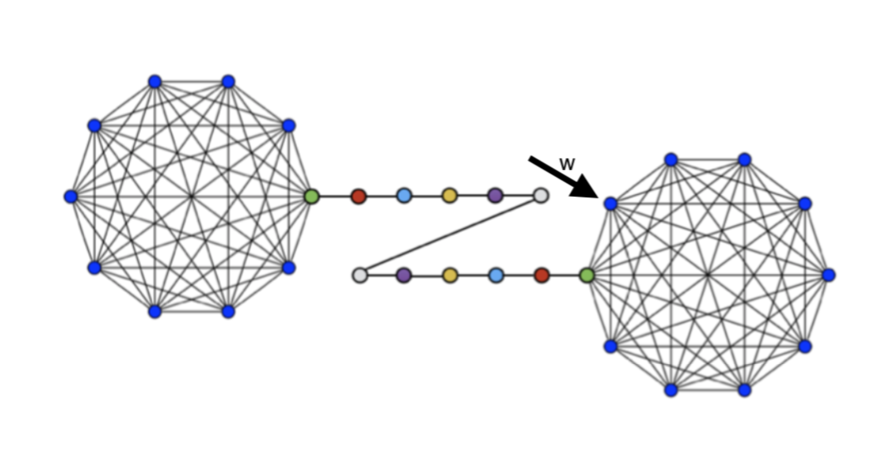
\includegraphics[width=0.6\columnwidth]{CS224W_Homework1/fig5.png}
  \caption{Two 10-node cliques}
  \label{fig:10-node}
\end{figure}

.\\\\\\\\
\subsection{ node2vec \& struct2vec (ii) (3 points)}
In the above figure \ref{fig:10-node}, suppose you arrive at node w. What are the nodes that you can reach after taking one step further with the node2vec algorithm? What about with the struct2vec algorithm (suppose that for this graph, $g_k(u, v) > 0$ for any u,v,k)?

\Solution{With node2vec, using a standard random walk (disregarding params p and q), there is a higher likelihood of staying within w's clique, simply because there are 9 possible ways to do so for each node in the clique, versus 1 way to travel to the other clique.
With struc2vec, if the path to the other clique is more heavily or lightly weighted than random due to structural dis/similarities, there is a higher/lower likelihood than random of travelling to nodes in the other clique.}

\subsection{node2vec \& struct2vec (iii) (3 points)}
Why is it necessary to consider different $g_k$'s during the random walk?

\Solution{So that emaphases on different graph features can be explored, e.g. degrees, cycles, short-range/long-range interactions,
 so that the struct2vec embeddings have richer set of features represented.}

\subsection{node2vec \& struct2vec (iv) (3 points)}
Characterize the vector representations (i.e. the embedding space) of the two 10-node cliques after running the struct2vec algorithm on the graph in the above figure (Figure \ref{fig:10-node}).

\Solution{Given that the graph in Figure 2.1 consists of two separate 10-node cliques connected by a single edge:
Nodes within each clique will have similar embeddings, especially those symmetric around the long edge between the cliques, and nodes in different cliques but playing a symmetrical role in their respective cliques.
Nodes along the connecting edge will be very different embeddings to the clique nodes, and larger variety amongst themselves depending on how close they are to another clique.}


\section{GCN (11 points)}

Consider a graph $G = (V, E)$, with node features $x(v)$ for each $v \in V$. For each node $v \in V$, let $h^{(0)}_v = x(v)$ be the node’s initial embedding. At each iteration $k$, the embeddings are updated as 

$$
\begin{aligned}
h_{\mathcal{N}(v)}^{(k)} & =\operatorname{AGGREGATE}\left(\left\{h_u^{(k-1)}, \forall u \in \mathcal{N}(v)\right\}\right) \\
h_v^{(k)} & =\operatorname{COMBINE}\left(h_v^{(k-1)}, h_{\mathcal{N}(v)}^{(k)}\right),
\end{aligned}
$$

\noindent for some functions $\operatorname{AGGREGATE}(\cdot)$ and $\operatorname{COMBINE}(\cdot)$. Note that the argument to the $\operatorname{AGGREGATE}(\cdot)$ function, ${h^{(k-1)}_u, \forall u \in \mathcal{N}(v)}$, is a \textit{multi-set}.
That is, since multiple nodes can have the same embedding, the same element can occur in ${h^{(k-1)}_u, \forall u \in \mathcal{N}(v)}$ multiple times.
Finally, a graph itself may be embedded by computing some function applied to the multi-set of all the node embeddings at some final iteration $K$, which we notate as 

$$\operatorname { READOUT }\left(\left\{h_v^{(K)}, \forall v \in V\right\}\right)$$

We want to use the graph embeddings above to test whether two graphs $G_1 = (V_1, E_1)$ and $G_2 = (V_2, E_2)$ are \textit{isomorphic}.
Recall that this is true if and only if there is some bijection $\phi : V_1 \rightarrow V_2$ between nodes of $G_1$ and nodes of $G_2$ such that for any $u, v \in V_1$, 
$$(u, v) \in E_1 \Leftrightarrow (\phi(u), \phi(v)) \in E_2$$

The way we use the model above to test isomorphism is the following. For the two graphs, if their readout functions differ, that is 

$$\operatorname { READOUT }\left(\left\{h_v^{(K)}, \forall v \in V_1\right\}\right) \neq \operatorname { READOUT }\left(\left\{h_v^{(K)}, \forall v \in V_2\right\}\right),$$

we conclude the graphs are \textit{not} isomorphic. Otherwise, we conclude the graphs are isomorphic. Note that this algorithm is not perfect: graph isomorphism is thought to be hard! Below, we will explore the expressiveness of these graph embeddings. 

\subsection{Isomorphism Check (2 points)}
Are the following two graphs isomorphic? If so, demonstrate an isomorphism
between the sets of vertices. To demonstrate an isomorphism between two
graphs, you need to find a 1-to-1 correspondence between their nodes and edges.
If these two graphs are not isomorphic, prove it by finding a structure (node
and/or edge) in one graph which is not present in the other. 
    \begin{figure}[H]
        \centering
        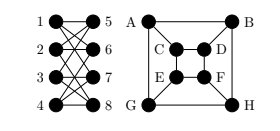
\includegraphics[width=0.5\textwidth]{CS224W_Homework1/fig1.png}
    \end{figure}

\Solution{
  
They are isomorphic: (A,B,C,D,E,F,G,H) maps to (1, 5, 6, 2, 4, 8, 7, 3).}


\subsection{Aggregation Choice (3 points)} 
The choice of the $\operatorname{AGGREGATE(\cdot)}$ is important for the expressiveness of the model above. Three common choices are: $$
\begin{aligned}
\operatorname{AGGREGATE}_{\max }\left(\left\{h_u^{(k-1)}, \forall u \in \mathcal{N}(v)\right\}\right)_i & =\max _{u \in \mathcal{N}(v)}\left(h_u^{(k-1)}\right)_i \text { (element-wise max)} \\
\operatorname{AGGREGATE}_{\text {mean}}\left(\left\{h_u^{(k-1)}, \forall u \in \mathcal{N}(v)\right\}\right) & =\frac{1}{|\mathcal{N}(v)|} \sum_{u \in \mathcal{N}(v)}\left(h_u^{(k-1)}\right) \\
\operatorname{AGGREGATE}_{\text {sum}}\left(\left\{h_u^{(k-1)}, \forall u \in \mathcal{N}(v)\right\}\right) & =\sum_{u \in \mathcal{N}(v)}\left(h_u^{(k-1)}\right)
\end{aligned}
$$
Give an example of two graphs $G_1 = (V_1, E_1)$ and $G_2 = (V_2, E_2)$ and their initial node features, such that for some node $v_1 \in V_1$ and some node $v_2 \in V_2$ with the same initial features $h^{(0)}_{v_1} = h^{(0)}_{v_2}$, the updated features $h^{(1)}_{v_1}$ and $h^{(1)}_{v_2}$ are equal if we use mean and max aggregation, but different if 
we use sum aggregation.\\
\textbf{Hint:} Your node features can be scalars rather than vectors, i.e. one dimensional node features instead of n-dimensional. Also, You are free to arbitrarily choose the number of nodes (e.g. 3 nodes), their connections (i.e. edges between
nodes) in your example.

\Solution{
For an example where the graphs have different structures and different node features:
Figures 3.1 and 3.2.

\begin{figure}
  \centering
  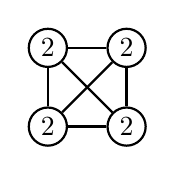
\begin{tikzpicture}
  \tikzstyle{v} = [circle, draw, thick, inner sep=2pt, fill=white]
  \tikzstyle{e} = [thick];
  \node[v](v1) at (0,0){2};
  \node[v](v2) at (0,1){2};
  \node[v](v3) at (1,1){2};
  \node[v](v4) at (1,0){2};

  \draw[e](v1)--(v2);
  \draw[e](v2)--(v3);
  \draw[e](v3)--(v4);
  \draw[e](v4)--(v1);
  \draw[e](v4)--(v2);
  \draw[e](v1)--(v3);

  \end{tikzpicture}
  \caption{$G_1$ with initial features, or features updated with mean/max aggregation.}
\end{figure}

\begin{figure}
  \centering
  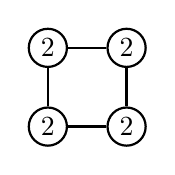
\begin{tikzpicture}
  \tikzstyle{v} = [circle, draw, thick, inner sep=2pt, fill=white]
  \tikzstyle{e} = [thick];
  \node[v](v1) at (0,0){2};
  \node[v](v2) at (0,1){2};
  \node[v](v3) at (1,1){2};
  \node[v](v4) at (1,0){2};

  \draw[e](v1)--(v2);
  \draw[e](v2)--(v3);
  \draw[e](v3)--(v4);
  \draw[e](v4)--(v1);

  \end{tikzpicture}
  \caption{$G_2$ with initial features, or features updated with mean/max aggregation.}
\end{figure}

With mean or max aggregation, the updated features of the two graphs all remain as 2.
With sum aggregation, $G_1$'s updated features all become 8, while $G_2$'s all become 6.
}


\subsection{Weisfeiler-Lehman Test (6 points)}
Our isomorphism-test algorithm is known to be at most as powerful as the well-known \textit{Weisfeiler-Lehman test} (WL test). At each iteration, this algorithm updates the representation of each node to be the set containing its previous representation and the previous representations of all its neighbors. The full algorithm is below.

    \begin{figure}[H]
        \centering
        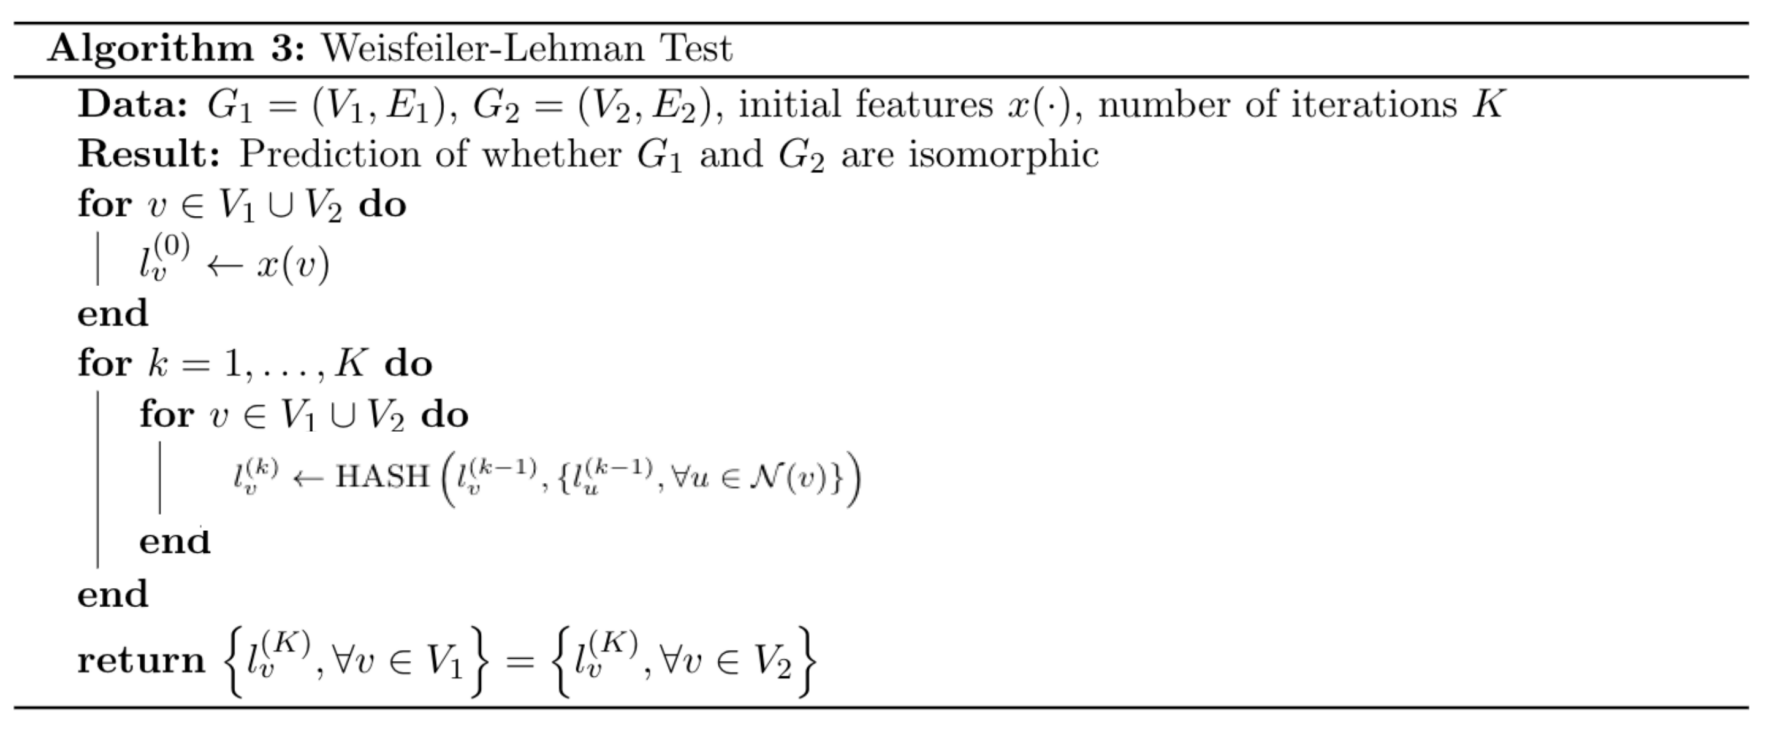
\includegraphics[width=1.0\textwidth]{CS224W_Homework1/algo-3.png}
    \end{figure}

    Prove that our neural model is at most as powerful as the WL test. More precisely, let $G_1$ and $G_2$ be non-isomorphic, and suppose that their node embeddings are updated over $K$ iterations with the same $\operatorname{AGGREGATE}(\cdot)$ and $\operatorname{COMBINE}(\cdot)$ functions. Show that if

    $$\operatorname { READOUT }\left(\left\{h_v^{(K)}, \forall v \in V_1\right\}\right) \neq \operatorname { READOUT }\left(\left\{h_v^{(K)}, \forall v \in V_2\right\}\right),$$

then the WL test also decides the graphs are not isomorphic.\\

Note: The proof has to be generic to any AGGREGATE, COMBINE, READOUT functions. Namely, it's not sufficient to show this for a specific instance of the GNN model.\\

\textbf{Hint:} You can use proof by contradiction by first assuming that \textit{Weisfeiler-Lehman} test cannot decide whether $G_1$ and $G_2$ are isomorphic at the end of $K$’th iteration.

\Solution{Given     $$\operatorname { READOUT }\left(\left\{h_v^{(K)}, \forall v \in V_1\right\}\right) \neq \operatorname { READOUT }\left(\left\{h_v^{(K)}, \forall v \in V_2\right\}\right),$$.
Now assume by way of contradiction that the WL test distinguish between $G_1$ and $G_2$ are isomorphic at the end of $K$’th iteration.
This implies that the multisets of representations (and thus the structural information they represent) are the same for both graphs at each iteration of the WL test up to K.
Then the neural model which uses the same AGGREGATE and COMBINE functions based on these representations, would produce identical embeddings for corresponding nodes in the two graphs.
Hence the READOUT function would give the same output for the two graphs. This contradicts our assumption. 
Conclude that if the READOUT gives different outputs for the two graphs, then the WL test can also tell that the graphs are not isomorphic.

}


\end{document}
